

\tikzset{every picture/.style={line width=0.75pt}} %set default line width to 0.75pt        

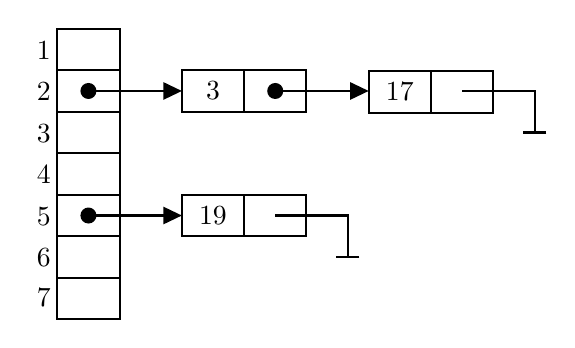
\begin{tikzpicture}[x=0.75pt,y=0.75pt,yscale=-1,xscale=1][H]
%uncomment if require: \path (0,181); %set diagram left start at 0, and has height of 181

%Shape: Rectangle [id:dp31075993805350643] 
\draw   (20,20) -- (50,20) -- (50,40) -- (20,40) -- cycle ;
%Shape: Rectangle [id:dp07786860939393403] 
\draw   (20,60) -- (50,60) -- (50,80) -- (20,80) -- cycle ;
%Shape: Rectangle [id:dp4591623739856949] 
\draw   (20,40) -- (50,40) -- (50,60) -- (20,60) -- cycle ;
%Shape: Rectangle [id:dp983416511512617] 
\draw   (20,80) -- (50,80) -- (50,100) -- (20,100) -- cycle ;
%Shape: Rectangle [id:dp04528718387197084] 
\draw   (80,40) -- (110,40) -- (110,60) -- (80,60) -- cycle ;
%Shape: Rectangle [id:dp1270001423171485] 
\draw   (20,140) -- (50,140) -- (50,160) -- (20,160) -- cycle ;
%Shape: Rectangle [id:dp776903324067578] 
\draw   (20,120) -- (50,120) -- (50,140) -- (20,140) -- cycle ;
%Shape: Rectangle [id:dp08008497435086515] 
\draw   (20,100) -- (50,100) -- (50,120) -- (20,120) -- cycle ;
%Shape: Rectangle [id:dp6528086235651709] 
\draw   (110,40) -- (140,40) -- (140,60) -- (110,60) -- cycle ;
%Shape: Rectangle [id:dp6043880104015285] 
\draw   (170,40.5) -- (200,40.5) -- (200,60.5) -- (170,60.5) -- cycle ;
%Shape: Rectangle [id:dp5461726616378066] 
\draw   (200,40.5) -- (230,40.5) -- (230,60.5) -- (200,60.5) -- cycle ;
%Shape: Rectangle [id:dp31723847172342756] 
\draw   (80,100) -- (110,100) -- (110,120) -- (80,120) -- cycle ;
%Shape: Rectangle [id:dp9818861995587984] 
\draw   (110,100) -- (140,100) -- (140,120) -- (110,120) -- cycle ;
%Straight Lines [id:da5730569526468681] 
\draw    (35,50) -- (77,50) ;
\draw [shift={(80,50)}, rotate = 180] [fill={rgb, 255:red, 0; green, 0; blue, 0 }  ][line width=0.08]  [draw opacity=0] (8.93,-4.29) -- (0,0) -- (8.93,4.29) -- cycle    ;
\draw [shift={(35,50)}, rotate = 0] [color={rgb, 255:red, 0; green, 0; blue, 0 }  ][fill={rgb, 255:red, 0; green, 0; blue, 0 }  ][line width=0.75]      (0, 0) circle [x radius= 3.35, y radius= 3.35]   ;
%Straight Lines [id:da6922082890770056] 
\draw    (125,50) -- (167,50) ;
\draw [shift={(170,50)}, rotate = 180] [fill={rgb, 255:red, 0; green, 0; blue, 0 }  ][line width=0.08]  [draw opacity=0] (8.93,-4.29) -- (0,0) -- (8.93,4.29) -- cycle    ;
\draw [shift={(125,50)}, rotate = 0] [color={rgb, 255:red, 0; green, 0; blue, 0 }  ][fill={rgb, 255:red, 0; green, 0; blue, 0 }  ][line width=0.75]      (0, 0) circle [x radius= 3.35, y radius= 3.35]   ;
%Straight Lines [id:da7299557815790314] 
\draw    (35,110) -- (77,110) ;
\draw [shift={(80,110)}, rotate = 180] [fill={rgb, 255:red, 0; green, 0; blue, 0 }  ][line width=0.08]  [draw opacity=0] (8.93,-4.29) -- (0,0) -- (8.93,4.29) -- cycle    ;
\draw [shift={(35,110)}, rotate = 0] [color={rgb, 255:red, 0; green, 0; blue, 0 }  ][fill={rgb, 255:red, 0; green, 0; blue, 0 }  ][line width=0.75]      (0, 0) circle [x radius= 3.35, y radius= 3.35]   ;
%Straight Lines [id:da4088411111836039] 
\draw    (125,110) -- (160,110) -- (160,130) ;
\draw [shift={(160,130)}, rotate = 270] [color={rgb, 255:red, 0; green, 0; blue, 0 }  ][line width=0.75]    (0,5.59) -- (0,-5.59)   ;

%Straight Lines [id:da04469814123042082] 
\draw    (215,50) -- (250,50) -- (250,70) ;
\draw [shift={(250,70)}, rotate = 270] [color={rgb, 255:red, 0; green, 0; blue, 0 }  ][line width=0.75]    (0,5.59) -- (0,-5.59)   ;


% Text Node
\draw (13.5,50.5) node   [align=left] {2};
% Text Node
\draw (13.5,30.5) node   [align=left] {1};
% Text Node
\draw (13.5,70.5) node   [align=left] {3};
% Text Node
\draw (13.5,90.5) node   [align=left] {4};
% Text Node
\draw (13.5,110.5) node   [align=left] {5};
% Text Node
\draw (13.5,130.5) node   [align=left] {6};
% Text Node
\draw (13.5,149.5) node   [align=left] {7};
% Text Node
\draw (95,50) node   [align=left] {3};
% Text Node
\draw (185,50.5) node   [align=left] {17};
% Text Node
\draw (95,110) node   [align=left] {19};


\end{tikzpicture}
